\section{Grundlagen}

\subsection{Smartphones und Marktentwicklung}
% Quellen: 
% Statistik Smartphones Deutschland - https://www.statista.com/statistics/461801/number-of-smartphone-users-in-germany/
% Smartphone History / Development - https://www.springerprofessional.de/a-brief-history-of-the-smartphone/16062424?searchResult=1.a%20brief%20history%20of%20the%20smartphone&searchBackButton=true&fulltextView=true

% Notizen:
% Hier mehrere Grafiken der Entwicklung einbinden (Statista)

% Ganz eventuell (eher generell Smartphone)
% Definition Smartphone - https://www.springerprofessional.de/smartphone-power-management-based-on-convlstm-model/18721566?searchResult=4.smartphone&searchBackButton=true&fulltextView=true

Der Markt für Smartphones in Deutschland ist in den letzten Jahren stark gewachsen. Im Jahr 2019 besaßen über 57 Millionen Menschen ein Smartphone.\footnote{\cite[Vgl.][]{Statista2020}} Auch die Übertragungstechnologien und Leistungsfähigkeit der mobilen Endgeräte haben sich positiv entwickelt. Durch eine hohe Verfügbarkeit und wachsende Bandbreiten haben Unternehmen heutzutage die Möglichkeit, mobile Geräte zur Vertriebsunterstützung einzusetzen. Vor allem die Ortsunabhängigkeit spielt dabei eine Rolle.\footnote{\cite[Vgl.][231--239]{Schmitz2021}}

\subsection{Mobile Anwendungen}
% Quellen:
% Definition Apps - https://www.springerprofessional.de/mobile-anwendungen-und-die-entwicklung-der-app-economy/18674004?searchResult=3.mobile%20app&searchBackButton=true&fulltextView=true

Das Wort App ist eine Abkürzung für das englische Wort \enquote{Application}. Zu deutsch bedeutet das Anwendungssoftware. Im Rahmen dieser Arbeit ist mit dem Begriff App eine Anwendung für mobile Endgeräte gemeint.\footnote{\cite[Vgl.][82]{Kollmann2020}}

% Heutzutage haben sich mobile Anwendungen weiterentwickelt. Damals hauptsächlich Kommunikation. Heute durch technologischen Fortschritt, Breitbandausbau neuer Stellenwert. Neue Mehrwerte.
% \footnote{\cite[Vgl.][1--4]{Aichele2016}}

\subsubsection{Plattformen}
% Quellen:
% https://gs.statcounter.com/os-market-share/mobile/

Für die Entwicklung einer App ist es wichtig, die zu unterstützenden Plattform früh in Betracht zu ziehen. Je nach Plattform unterscheiden sich die Herangehensweisen an die Entwicklung (siehe \ref{sec:mobile_app_types}). In Abbildung \ref{fig:mobile_os_market_share} sind alle Betriebssysteme im mobilen Bereich nach ihrem weltweiten Marktanteil in den vergangenen 10 Jahren aufgeschlüsselt. Man kann erkennen, dass Android von Google (orange Linie) sich seit fast acht Jahren auf der Position des Marktführers befindet. Heute besitzt Android demnach einen Marktanteil von {71,93\%}. Danach folgt iOS, welches eine relativ stetige Entwicklung hinter sich hat und heute {27,47\%} ausmacht. Die anderen Betriebssysteme wie Symbian, Samsung Tizen, BlackBerry OS oder Series 40 sind mittlerweile kaum noch relevant oder Nischenprodukte. Windows Phone wird seit Ende 2019 nicht mehr unterstützt.\footnote{\cite[Vgl.][83]{Kollmann2020}} Mit der Entwicklung einer App für die Plattformen Android und iOS kann man heutzutage über {99\%} aller Nutzer bedienen.

\begin{figure}[hbt]
    \centering
    \begin{minipage}[t]{.7\textwidth}
        \caption{Mobile Operating System Market Share Worldwide - January 2021}
        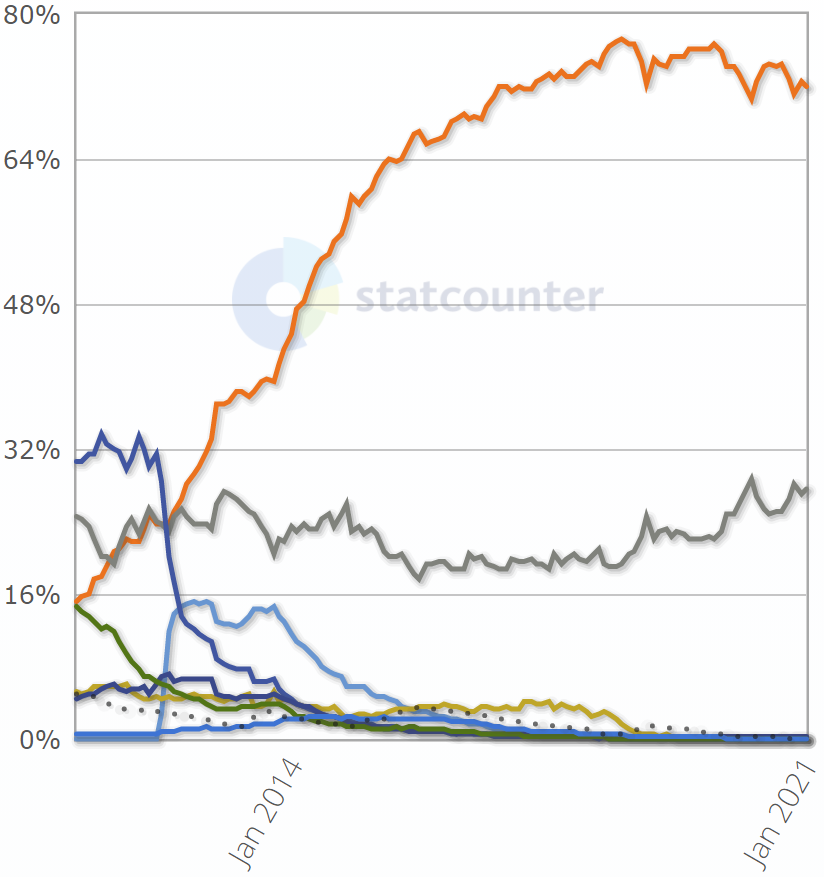
\includegraphics[width=1\textwidth]{img/Mobile_OS_MarketShare.png}\\
        \source{\cite{Statcounter2021}}
        \label{fig:mobile_os_market_share}
    \end{minipage}
\end{figure}

%\subsubsection{User Experience}
% Quellen:
% UX (agile UX Entwicklung, Personas, Befragungen) - https://www.springerprofessional.de/user-experience-verstehen/18509082?searchResult=4.User%20Experience&searchBackButton=true&fulltextView=true
% UX Gesichtspunkte - https://www.springerprofessional.de/adaptive-user-experience-und-empathische-hmi-konzepte/18513822?searchResult=1.User%20Experience&searchBackButton=true&fulltextView=true
% Performance - https://www.springerprofessional.de/analysing-the-performance-of-mobile-cross-platform-development-a/18203138?searchResult=2.cross%20platform%20app&searchBackButton=true&fulltextView=true

\subsubsection{Arten von mobilen Anwendungen}
\label{sec:mobile_app_types}

Im folgenden werden die Vor- und Nachteile der verschiedenen Arten von Apps aufgegriffen und kurz verglichen. Die Aspekte basieren auf der Ausführung von \cite{Kollmann2020}\footnote{\cite[Vgl.][84--87]{Kollmann2020}}.

\paragraph{Native Anwendungen}
Eine native Anwendung wird für eine einzelne Plattform entwickelt. Mit dem \gls{SDK} stellt der Herausgeber der Plattform Werkzeuge, Komponenten und Schnittstellen für Entwickler bereit. Mithilfe dieser und den unterstützten Programmiersprachen kann dann eine App entwickelt werden. Für die Plattform Android können z. B. die Programmiersprachen Java, Kotlin und C++ genutzt werden.\footnote{\cite[Vgl.][]{AndroidDocumentation2021a}} Anwendungen für iOS werden in Objective-C oder Swift programmiert.\footnote{\cite[Vgl.][]{SwiftDocumentation2021}} Über Schnittstellen wird der direkte Zugriff auf Hardwareressourcen wie Kamera, Mikrofon oder die Standortbestimmung ermöglicht. Das \gls{SDK} wird mit jeder neuen Betriebssystemversion aktualisiert und ermöglicht damit die sofortige Nutzung neuer Funktionalitäten. Durch ihre Nähe zum Betriebssystem eignen sich native Anwendungen für rechen- oder grafikintensive Aufgaben. Werden die plattformspezifischen \gls{UI}-Standardelemente (z. B. Schaltflächen, Textfelder und Schriftarten) des \gls{SDK} genutzt, kann das Design der App an das des Betriebssystems angepasst werden. Es entsteht eine vertraute Umgebung für die Benutzer. Native Anwendungen und deren Updates werden größtenteils über die offiziellen Märkte der jeweiligen Plattform vertrieben. Unter Android ist das der \enquote{Google Play Store}. Unter iOS hingegen der \enquote{App Store}. Native Anwendungen benötigen zum Starten keine Internetverbindung, da die Software auf die Endgeräte heruntergeladen und installiert wird. Um mehrere Plattformen zu unterstützten, müssen separate Anwendungen entwickelt werden. Dies führt zu erhöhten Kosten. Durch die Nutzung von Cross-Platform Frameworks können Apps entwickelt werden, die sich in native Anwendungen für mehrere Plattformen kompilieren lassen. Diese Frameworks sind allerdings nicht immer auf dem neusten Entwicklungsstand aller Plattformen und besitzen eine eingeschränkte Unterstützung von Plattformfunktionalitäten\footnote{\cite[Vgl.][]{XamarinDocumentation2021}}

%+ Design der App an die Eigenheiten eines Betriebssystems
%+ User Experience (Schnell)
%+ Performance (Volle Nutzung der Kerne, Animationen, Reaktiv)
%+ Direkter Zugriff auf Systemressourcen (Kamera, Mikrofon, Speicher)
%+ Vertrautheit durch den Nutzer (selbe Schaltflächen, Standardelemente etc.)
%+ Einmal runtergeladen benötigt sie keine Internetverbindung
%- Läuft nur auf einer Plattform
%- Höhere Entwicklungskosten
%- Braucht mehr Entwickler und hat in Zukunft höheren Wartungsaufwand
%- Um den gesamten Markt mitzunehmen müssen Android und iOS unterstützt werden (Statista Referenz!)

\paragraph{Webanwendungen}
Webanwendungen sind mobile Anwendungen, welche über einen Webbrowser aufgerufen werden können. Sie werden nicht auf dem Gerät installiert und benötigen daher eine Internetverbindung, um sie zu starten. Webanwendungen sind plattformunabhängig. Jedes Endgerät mit einem Webbrowser kann sie ausführen. Sie werden in \gls{HTML}, \gls{JS} und \gls{CSS} geschrieben. Der Nutzer lädt bei jedem Start die neuste Version der Anwendung. Updates müssen nicht über die Plattformmärkte ausgeteilt werden. Allerdings kann diese Art einer Anwendung auch nicht die Werbe- und Monetarisierungsmöglichkeiten der Märkte nutzen. Da Webanwendungen innerhalb eines Browsers ausgeführt werden, sind Systemressourcen begrenzt und der Zugriff auf Hardware nur teilweise möglich. Außerdem haben Webanwendungen keinen Zugriff auf die Standardkomponenten der jeweiligen Plattform. Dadurch entsteht eine systemfremde Benutzeroberfläche.

%+ Website im App-Mantel
%+ Vorhandenes Wissen im Web-Bereich kann genutzt werden
%+ Bietet Bridge Funktionalität für die Nutzung von GPS, Kamera etc.
%+ Eine Entwicklung für alle Plattformen
%+ Kostengünstiger in der späteren Wartung
%- Feinheiten müssen doch wieder einzeln für die jeweilige Plattform ausgearbeitet werden
%- Durch den Mantel laufen sie eventuell langsamer
%- Komponenten sehen eventuell anders aus (Buttons etc.)
%- Muss sich trotzdem mit Verschiedenheiten auseinandersetzen (verschiedene Navigationsmöglichkeiten, unterstützte Hardware-Features)

\paragraph{Hybride Anwendungen}
Hybride Anwendungen werden ebenfalls wie Webanwendungen entwickelt. Diese wird dann allerdings in einer nativen App eingebettet. Dadurch kann die Anwendung auf den Endgeräten installiert werden und benötigt keine Internetverbindung. Außerdem können die Vorteile der Plattformmärkte für den Vertrieb genutzt werden. Diese Anwendungen sind ebenfalls durch die Ressourcenlimits der Browser begrenzt. Über die native Hülle lassen sich dafür Zugriffe auf Hardwareressourcen ermöglichen.

%+ Zusammenschluss der beiden Welten

\subsection{Android}
Android ist ein Software-Stack\footnote{Eine Zusammenfassung von Software, die aufeinander aufbaut}, dessen Quellcode offen vorliegt (Open-Source). Es unterstützt eine breite Palette an Geräteklassen und kann von den Hardwareherstellern auf ihre Geräte zugeschnitten und angepasst werden. Ziel von Android ist die Entwicklung einer offenen Plattform für Telekommunikationsanbieter, \glspl{OEM}\footnote{zu deutsch: Erstausrüster. Firmen, die Hardware herstellen, diese aber nicht selber in den Einzelhandel bringen. Beispiel: Prozessorhersteller für Smartphones} und Softwareentwickler, um gemeinsam Entwicklungen und Innovationen voranzutreiben.\footnote{\cite[Vgl.][]{AndroidDocSetup2020}} Heutzutage ist Android auf Fernsehern, in Autos, Uhren, eBook Readern, Netbooks, Spielekonsolen und Smartphones im Einsatz. Für den Zugriff auf Netzwerk, Speicher und andere Hardware stellt die Android-Plattform Schnittstellen zur Verfügung, die auch über Updates hinweg einheitlich bleiben.\footnote{\cite[Vgl.][1--4]{Hagos2020}}

\subsubsection{Entwicklungswerkzeuge und Bibliotheken}
% Quellen:
% Android Versionsverteilung (eventuell eigene Grafik aus Android Studio) - https://www.statista.com/statistics/271774/share-of-android-platforms-on-mobile-devices-with-android-os/

% Download von weiteren Tools, SDK Download und Updates, Debugging, Bietet Hilfen während der Entwicklung, Verbesserungsvorschläge, Auto Vervollständigungen, Projektansicht, Verwalten von Ressourcen, Logs auslesen, WYSIWYG Editor für Layouts, Hinzufügen externer Bibliotheken

Die offizielle Entwicklungsumgebung für Android ist das \enquote{Android Studio}. Über sie können Entwickler das \gls{SDK}, \gls{USB}-Treiber und externe Bibliotheken von Google herunterladen.\footnote{\cite[Vgl.][10--14]{Hagos2020}} Während der Entwicklung gibt Android Studio Tipps und Hilfen, um die Entwicklung für mehrere Android-Versionen zu erleichtern. Außerdem können Ressourcen wie Bilder und Dateien für die App verwaltet werden. Um die Fehlerbehandlung zu erleichtern, gibt es zudem einen eingebauten Debugger und die Möglichkeit, Geräteprotokolle auszulesen. Die Gestaltung der Benutzeroberflächen erfolgt in \gls{XML} Dateien. Dafür bringt Android Studio einen eingebauten visuellen Editor mit.\footnote{\cite[Vgl.][33--37]{Hagos2020}} Im Anhang auf Seite \pageref{fig:android_studio_layout_editor} in Abbildung \ref{fig:android_studio_layout_editor} ist zu sehen, wie zwischen den beiden Ansichten gewechselt werden kann.

Wie in Abbildung \ref{fig:android_version_fragmentation} zu sehen ist, kommen zwar immer neue Android-Versionen auf den Markt, aber nicht alle Geräte am Markt sind auf dem neusten Stand. Im Jahr 2013 nutzten noch {69,2\%} aller Android-Geräte die neuste Version 4.x. Dagegen lag im ersten Halbjahr 2019 die Nutzung der Versionen 5.1.x bis 9 zwischen {7,8\%} und {16,9\%} je Version und damit relativ verstreut. Trotz der Veröffentlichung von Android 10 im Jahr 2020 nutzten immer noch {11,2\%} aller Geräte Android 6.0. Diese Fragmentierung entsteht dadurch, dass Gerätehersteller nur über einen begrenzten Zeitraum Updates für ihre Geräte liefern. Entwickler müssen demnach eine Vielzahl an Versionen unterstützen, um möglichst viele Nutzer ansprechen zu können. Um den Entwicklern diese Arbeit zu erleichtern, hat Google die AndroidX Bibliotheken entwickelt. Diese müssen separat in das App-Projekt eingebunden werden. Sie ermöglichen die Nutzung neuer Funktionen auf älteren Android-Versionen. Zusätzlich bieten sie nützliche Funktionalitäten, die nicht im \gls{SDK} verfügbar sind und die Entwicklung erleichtern.\footnote{\cite[Vgl.][]{AndroidSupportLibrary2020}}

\begin{figure}[hbt]
    \centering
    \begin{minipage}[t]{.8\textwidth}
        \caption{Android operating system share worldwide by OS version from 2013 to 2020}
        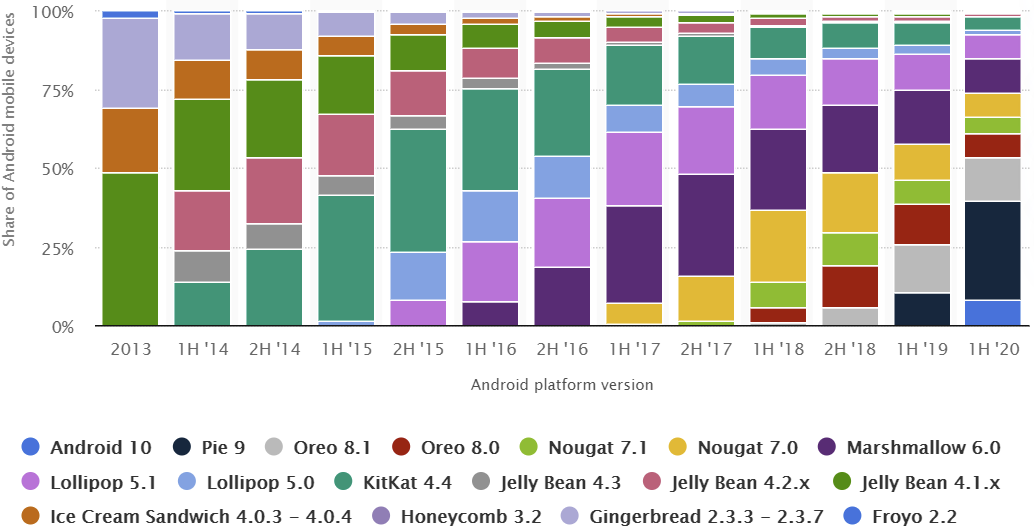
\includegraphics[width=1\textwidth]{img/Android_Version_Fragmentation.PNG}\\
        \source{\cite{StatistaAndroidVersion2020}}
        \label{fig:android_version_fragmentation}
    \end{minipage}
\end{figure}

\subsubsection{Komponenten einer Anwendung}
% Fragments / Activities
% XML Files und dann Java oder Kotlin

In diesem Unterkapitel sollen die technischen Bauteile einer Android-App beschrieben werden. Das Aussehen einiger Komponenten und deren Nutzung werden in Zusammenhang mit den Designrichtlinien im Kapitel \ref{sec:material_design} beschrieben.

Die Kernbausteine einer Android-App sind \enquote{Activities} und \enquote{Fragments}. Eine Activity besteht aus verschiedenen Elementen wie Textfeldern, Schaltflächen, Bilder und Fragments. Eine Anwendung kann aus mehreren Activities bestehen, die untereinander kommunizieren können. Es ist aber immer nur eine sichtbar. Fragments können ebenfalls Benutzerelemente enthalten. Sie müssen allerdings in einer Activity eingebettet werden. Dafür können mehrere Fragmente parallel oder verschachtelt dargestellt werden.\footnote{\cite[Vgl.][48\psq]{Hagos2020}} Durch die Nutzung von Fragments entstehen wieder verwendbare Teilelemente. So kann eine Benutzeroberfläche modularisiert werden.\footnote{\cite[Vgl.][]{AndroidFragments2020}} Google empfiehlt die Nutzung von wenigen Activities. Die Navigation in der App sollte stattdessen durch das Austauschen von Fragments implementiert werden. Um diesen Prozess zu vereinfachen, bietet sich die von Google entwickelte Bibliothek \enquote{Navigation component} an.\footnote{\cite[Vgl.][]{AndroidNavigationComponent2020}} Bei der Arbeit mit Activities und Fragments muss darauf geachtet werden, dass diese vom Android-System verwaltet werden. Das System kann diese Komponenten jederzeit zerstören und neu anlegen. Dies ist z. B. der Fall beim Rotieren des Geräts oder der Freigabe von Ressourcen durch das System. Jegliche Daten, die innerhalb dieser Komponenten gehalten werden, gehen dann verloren. Eine Methode um Daten außerhalb von diesen Elementen zu halten sind \enquote{ViewModel}. Diese werden in Kapitel \ref{sec:programmarchitektur} erläutert.

\subsubsection{Unterstützung mehrerer Geräteklassen}
\label{sec:geraeteklassen}
% Pixel Density
% APK und App Bundle Format

Android funktioniert auf einer Vielzahl von Geräten mit jeweils verschiedenen Bildschirmgrößen und Pixeldichten. Die Pixeldichte wird in \gls{DPI} gemessen. Das kann zu Schwierigkeiten bei der Entwicklung von Apps für alle Bildschirmgrößen führen. Um dies zu erleichtern, hat Android die \gls{DIP} eingeführt. Je nach \gls{DPI} werden diese unterschiedlich auf reale Bildschirmpixel skaliert. Am Beispiel eines Bildes ist dieses Vorgehen in Abbildung \ref{fig:android_dip_scaling} dargestellt. Auf Geräten mit einer Pixeldichte von bis zu 160 \gls{DPI} wird das Bild in seiner originalen Auflösung dargestellt. Bei einer Pixeldichte zwischen 160 und 240 \gls{DPI} wird die Breite und Höhe mit dem Faktor {1,5} skaliert. Bei größeren Pixeldichten bis zum Faktor 4. Da bei der Vergrößerung von Bildern häufig die Qualität abnimmt, können auch manuell Bilder für die jeweiligen Geräteklassen fest hinterlegt werden. Dafür muss eine von Android vorgegebene Ordnerstruktur verwendet werden (siehe Anhang Abbildung \ref{fig:android_dip_folder_structure} auf Seite \pageref{fig:android_dip_folder_structure} für ein Beispiel). Das Android-System wählt dann zur Laufzeit die Ressource nach der Klasse des Gerätes.\footnote{\cite[Vgl.][]{AndroidScreenDensities2020}}

\begin{figure}[hbt]
    \centering
    \begin{minipage}[t]{.8\textwidth}
        \caption{Relative sizes for bitmaps at different density sizes}
        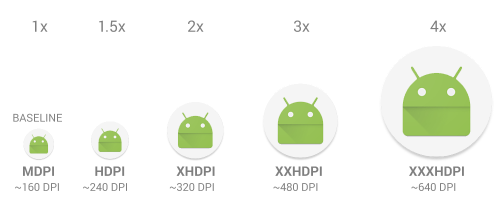
\includegraphics[width=1\textwidth]{img/DIP_Scaling.PNG}\\
        \source{\cite{AndroidScreenDensities2020}}
        \label{fig:android_dip_scaling}
    \end{minipage}
\end{figure}

\subsubsection{Anwendungsarchitektur}
\label{sec:programmarchitektur}
% Koin
% ViewModels testen

% DataBinding

% MVVM:
% View: Navigation, Manipulation der Elemente
% Model: Datenbasis (Repositories, Static Data, Daten aus einer Datei, Datenbank, Web-Service)
% ViewModel: Vermittler zwischen den beiden (lädt Daten in ein Model und bereitet sie für die View vor)

In Android können ViewModels genutzt werden, um Daten über die Neuerstellung von Activities und Fragments hinweg zu halten. Dafür kann einfach eine neue Klasse in Kotlin oder Java definiert werden, welche von der Klasse \enquote{ViewModel} erbt. Dieser ViewModel Typ kann dann aus einer Activity oder einem Fragment vom Android-System angefragt und verwendet werden. Die ViewModel Instanz bleibt bis zum manuellen Schließen der Activity oder des Fragments erhalten. ViewModels werden auch häufig verwendet, um Logik aus der View herauszubrechen.\footnote{\cite[Vgl.][210\psqq]{Hagos2020}}

Zusammen mit ViewModels eignet sich der Einsatz von \enquote{DataBinding}. DataBinding stellt eine Verbindung zwischen einer Eigenschaft und der Benutzeroberfläche her. Wenn sich der Wert der Eigenschaft aktualisiert, dann spiegelt sich dies automatisch in der Ansicht wider. DataBinding wird unter Android häufig mit \enquote{LiveData} Objekten aus der AndroidX Bibliothek umgesetzt. Diese können wie Variablen im ViewModel definiert werden. Sie enthalten einen bestimmten Typ. Durch die Registrierung eines Observers kann aus einer Activity oder einem Fragment auf Änderungen in dem LiveData Objekt reagiert werden. Durch die Nutzung von \enquote{ViewBinding} können LiveData Objekte direkt aus den XML-Layout Dateien angesprochen werden. Dann muss kein Code in der Activity geschrieben werden.\footnote{\cite[Vgl.][214\psqq]{Hagos2020}}

\subsubsection{Gestaltung der Benutzeroberfläche}
\label{sec:material_design}
% Abweichungen zu iOS
% Bottom Navigation
% Design generell
% Farbkontraste, Schatten, Schriftarten, Standard Elemente
% Einheitliche Elemente: Beispiel Buttons für Vor und Zurück

Android-Nutzer erwarten, dass eine Anwendung so aussieht und sich so verhält, wie es der Plattform entspricht.\footnote{\cite[Vgl.][]{AndroidDocDesign2019}} Für das visuelle Design hat Google das \enquote{Material Design} entworfen. Bei diesem handelt es sich um einen Leitfaden zur Umsetzung einer guten Benutzererfahrung und eines einheitlichen Designs. Dieses kann auch auf iOS und Webseiten angewendet werden. Google liefert dafür z. B. Artikel über Barrierefreiheit, Farbgestaltung, Typografie und die Nutzung von Symbolen. Außerdem stellt Google für mehrere Plattformen Bibliotheken mit vorgefertigten Komponenten bereit, die die Entwicklung anhand dieser Richtlinien einfacher gestalten. Beispiele sind Schaltflächen und Textfelder. Auch Kombinationen aus verschiedenen Elementen sind möglich. Durch die Nutzung von Schaltflächen, Texten und Bildern verbindet die \enquote{Card}-Komponente alle Informationen und Aktionen zu einem einzelnen Thema in einer Komponente. Im Anhang auf Seite \pageref{fig:material_card_example} in der Abbildung \ref{fig:material_card_example} ist beispielhaft der Aufbau einer solchen Komponente zu sehen.\footnote{\cite[Vgl.][]{MaterialFoundation2021}}

Auch zu der Navigation innerhalb einer Anwendung gibt das Material Design Hinweise. Seiten und Inhalte, die klar voneinander abgegrenzt werden können, können in einer \enquote{Bottom Navigation Bar} (zu deutsch: untere Navigationsleiste) untergebracht werden. Die auch in der Abbildung \ref{fig:material_bottom_nav_example} im Anhang auf Seite \pageref{fig:material_bottom_nav_example} zu sehende Leiste sollte niemals ausgeblendet werden. Sie dient als Navigation zwischen primären Zielen, die von überall aus der Anwendung erreichbar sein sollen. Außerdem sollten mindestens zwei bis maximal fünf Elemente auf dieser zu sehen sein. Sollten zu vielen Elemente dargestellt werden, verliert die Komponente an Übersichtlichkeit. Ein Element besteht dabei immer aus einem Symbol und einem optionalen Text. Dadurch, dass die Navigationsleiste am unteren Rand sehr gut mit einem Daumen erreichbar ist, fördert sie die Ergonomie. Weiterhin stellt die Leiste eine Konsistenz in der App dar, auf die der Nutzer von jeder Seite zugreifen kann.\footnote{\cite[Vgl.][]{MaterialBottomNav2021}}

Eine weitere wichtige Komponente ist die \enquote{Top app bar}. Diese bezieht sich immer auf den Kontext der aktuellen Seite. Links sollte sich ein Element befinden, um zu der vorherigen Seite zu navigieren, falls dies möglich ist. Dann der Titel der aktuellen Seite. Als letztes Aktionen, die im Kontext der aktuellen Seite möglich sind. Das kann z. B. eine Such- oder Filterfunktion sein. Ein Beispiel der Aufteilung findet sich im Anhang in Abbildung \ref{fig:material_top_bar_example} auf Seite \pageref{fig:material_top_bar_example}.\footnote{\cite[Vgl.][]{MaterialTopBar2021}}

Farben sind bei der Entwicklung einer App ebenfalls ein zentrales Thema. Sie können genutzt werden, um eine Markenpräsenz aufzubauen, den Fokus auf bestimmten Elemente zu rücken oder Elementzustände anzuzeigen. Durch die Nutzung weniger Farben auf Oberflächen können Bilder und Text in den Fokus gerückt werden. Durch die einheitliche Einfärbung von Schaltflächen, Fortschrittsindikatoren und Kontrollfeldern kann eine Markenpräsenz gestärkt werden.\footcite[Vgl.][]{MaterialColor2021}

\clearpage